\section{Le rôle de la température}

\subsection{Température et changement climatique}

Devenu incontesté dans la communauté scientifique, le réchauffement climatique
affecte la planète et ses systèmes biologiques à tous les niveaux
d'organisation \autocites{sagarin1999a,sala2000a,ipcc2007a,walther2002a}. Les
prédictions actuelles, regroupées et validées par le Groupe d’experts
Intergouvernemental sur \'{E}volution du Climat, projettent une augmentation de
la température moyenne à la surface du globe de 2 à 8$\degres$C d'ici à la fin
du siècle \autocites{ipcc2007a}. Ce changement de température sera resenti
différemment suivant les régions du globe, avec par exemple un réchauffement
plus prononcé aux pôles qu'à l'équateur. 

Des études sur le long terme ont montré que ces changements de température
peuvent modifier la distribution des traits d'histoires de vie dans les
populations naturelles \autocites{parmesan2006a,ozgul2009a}, mais également leur
distribution géographique, leur activité ou leur phénologie
\autocites{parmesan2006a,walther2002a}.
Face à ces changements déjà engagés et à ceux à venir, il est important de
comprendre et prédire l'impact que peuvent avoir la température et ses
changements sur la dynamique des populations \autocite{lavergne2010a}. 

\subsection{Les effets de la températures sur les individus}

Une population étant constituée de ses individus, il faut connaître les effets
de la température sur les individus pour comprendre les répercussions sur les
populations. 

Selon la règle de \textcites{bergmann1848a}, l'application de la thermodynamique
aux organismes endothermes prédit que les individus grandissent moins dans un
environnement chaud que dans un environnement froid. En effet, la perte de
chaleur se fait par la surface de l'individu alors que sa production se fait
proportionnellement à son volume. En environnement chaud, il est donc avantageux
d'avoir une petite taille pour maximiser son rapport surface sur volume et
favoriser ainsi la perte de chaleur. A l'inverse, en environnement froid, une
plus grande taille confère un avantage en réduisant proportionnellement la perte
de la chaleur produite par le corps. Cette règle a été énoncée pour les organismes produisant
leur propre chaleur et a été effectivement vérifiée en comparant les tailles
d'un grand nombre d'espèces de mammifères et leur température moyenne de vie. 

Cependant, de façon plus surprenante, les organismes ectothermes suivent eux
aussi une règle similaire et tendent également à avoir une plus petite taille
corporelle adulte dans des environnements plus chauds
\autocites{angilletta2009a,ohlberger2013a}.
Cette plasticité qui s'observe autant à l'échelle intra-spécifique
qu'inter-spécifique est appelée la règle taille--température
\autocites[``\textbf{temperature--size rule}''][]{atkinson1994a}. Celle-ci
suggère donc que les arguments thermodynamiques avancés par Bergmann ne sont probablement pas les seuls à conduire à une réduction de la taille corporelle en environnement chaud
\autocite{edeline2013a}.

Dans une revue parue récemment, \textcite{ohlberger2013a} fait le point sur les
implications de la température du niveau de l'individu et de sa physiologie à
celui de la communauté. Une première observation est que la température agit sur
la taille corporelle par l'intermédiaire de son action sur les réactions
biochimiques, et notamment celles issues du métabolisme et de l'acquisition des
ressources. La relation entre la vitesse des réactions biochimiques et la
température n'est pas linéaire, le taux de réaction augmente régulièrement avec
la température jusqu'à un optimum puis diminue très rapidement, conduisant à une
sensibilité asymétrique à la température \autocites{hochachka2002a,
angilletta2009a}. Il existe donc un compromis entre performance à basse et haute
température, et se spécialiser sur une température donnée n'est possible qu'au
détriment des autres \autocites{angilletta2009a}.

\begin{figure}[!ht] % Figure 1 
\centering
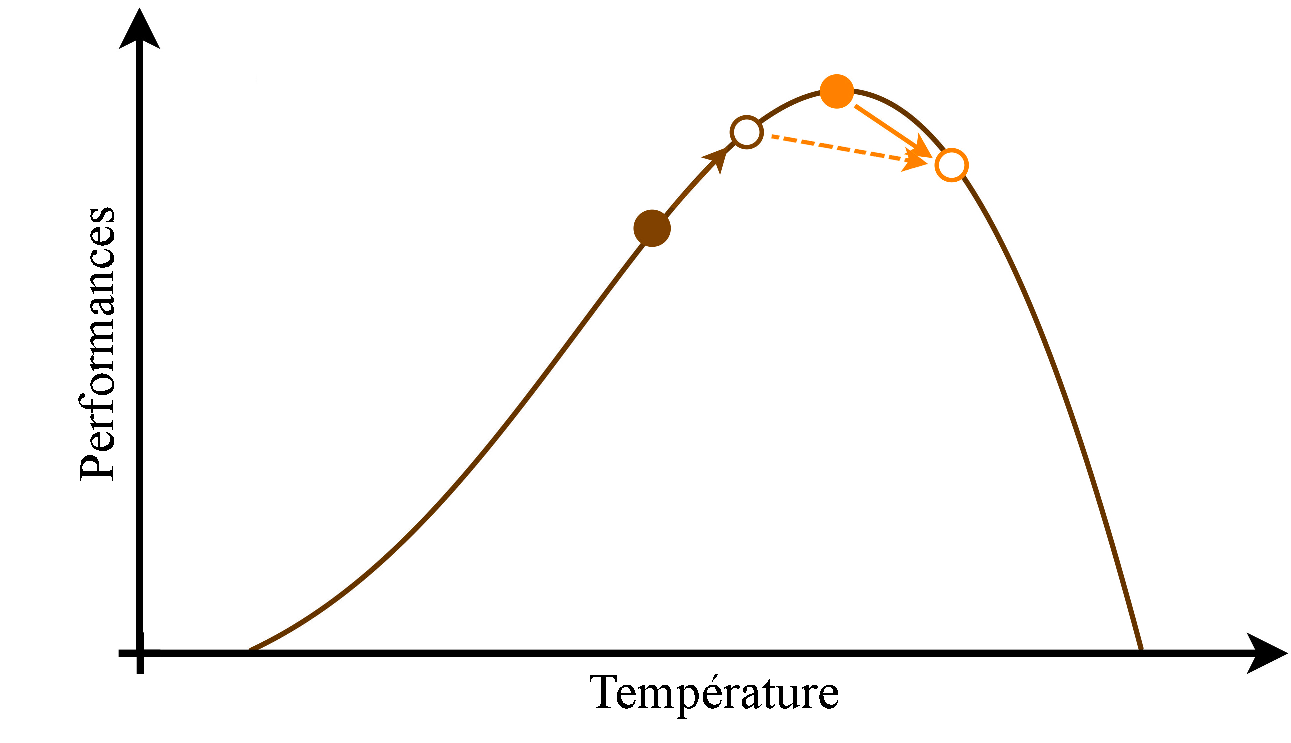
\includegraphics[width=0.66\textwidth]{1_CorpsDeThese/EA/Fig/ThermalCurve.pdf}
\caption[\lofimage{1_CorpsDeThese/EA/Fig/ThermalCurve.pdf}
Performance théorique en fonction de la température]{Performance théorique en
fonction de la température. D'après \textcites{ohlberger2013a}, Figure 1. Un
réchauffement du climat améliore les performances d'un individu qui vit dans
des conditions sous optimales si le changement est de petite amplitude (flèche
marron). Si l'individu est à l'optimum (point orange plein), le réchauffement
lui fait diminuer ses performances (flèche orange pleine). Si le changement est
de trop grande amplitude, les performances diminuent également (point marron
vide, flèche orange pointillée)}
\label{Fig:EA1}
\end{figure}

Cette sensibilité asymétrique à la température se répercute ensuite au niveau
de l'individu dans son ensemble, et en particulier sur son taux de croissance.
Ainsi, pour un individu vivant à une température sous-optimale, une augmentation
de température sera bénéfique alors qu'elle sera néfaste pour un individu vivant
déjà à sa température optimale. De même, si l'amplitude de l'augmentation est
trop importante, la température peut dépasser l'optimum et le réchauffement a
alors un effet néfaste . Ceci est illustré par la Figure
\ref{Fig:EA1}, d'après \textcites{ohlberger2013a}. Cependant, les individus sont
souvent capable d'adapter leur sensibilité à la température par plasticité
phénotypique. Ces réponses plastiques peuvent alors différer suivant la
fréquence et la longueur des changements de température
\autocites{angilletta2009a, huey1999a}.

Lorsque les températures subies par les individus ne dépassent pas la
température optimale (Figure \ref{Fig:EA1}), la plupart des ectothermes suivent
alors règle taille--température déjà énoncée \autocite{atkinson1994a}. Au cours
du développement, une température plus élevée entraîne alors une augmentation du
taux de croissance mais une diminution de la taille adulte (Figure
\ref{Fig:EA2}).
Si l'on s'intéresse à un âge ou un stade particulier (par exemple la
maturation), on observe alors une modification de la taille corporelle
correspondant à cet âge ou ce stage (par exemple, maturation à une taille plus
petite ou plus grande). Le suivi de ces modifications avec la
température permet de déterminer précisément les normes de réaction à la
température.

\begin{figure}[!ht] % Figure 1 
\centering
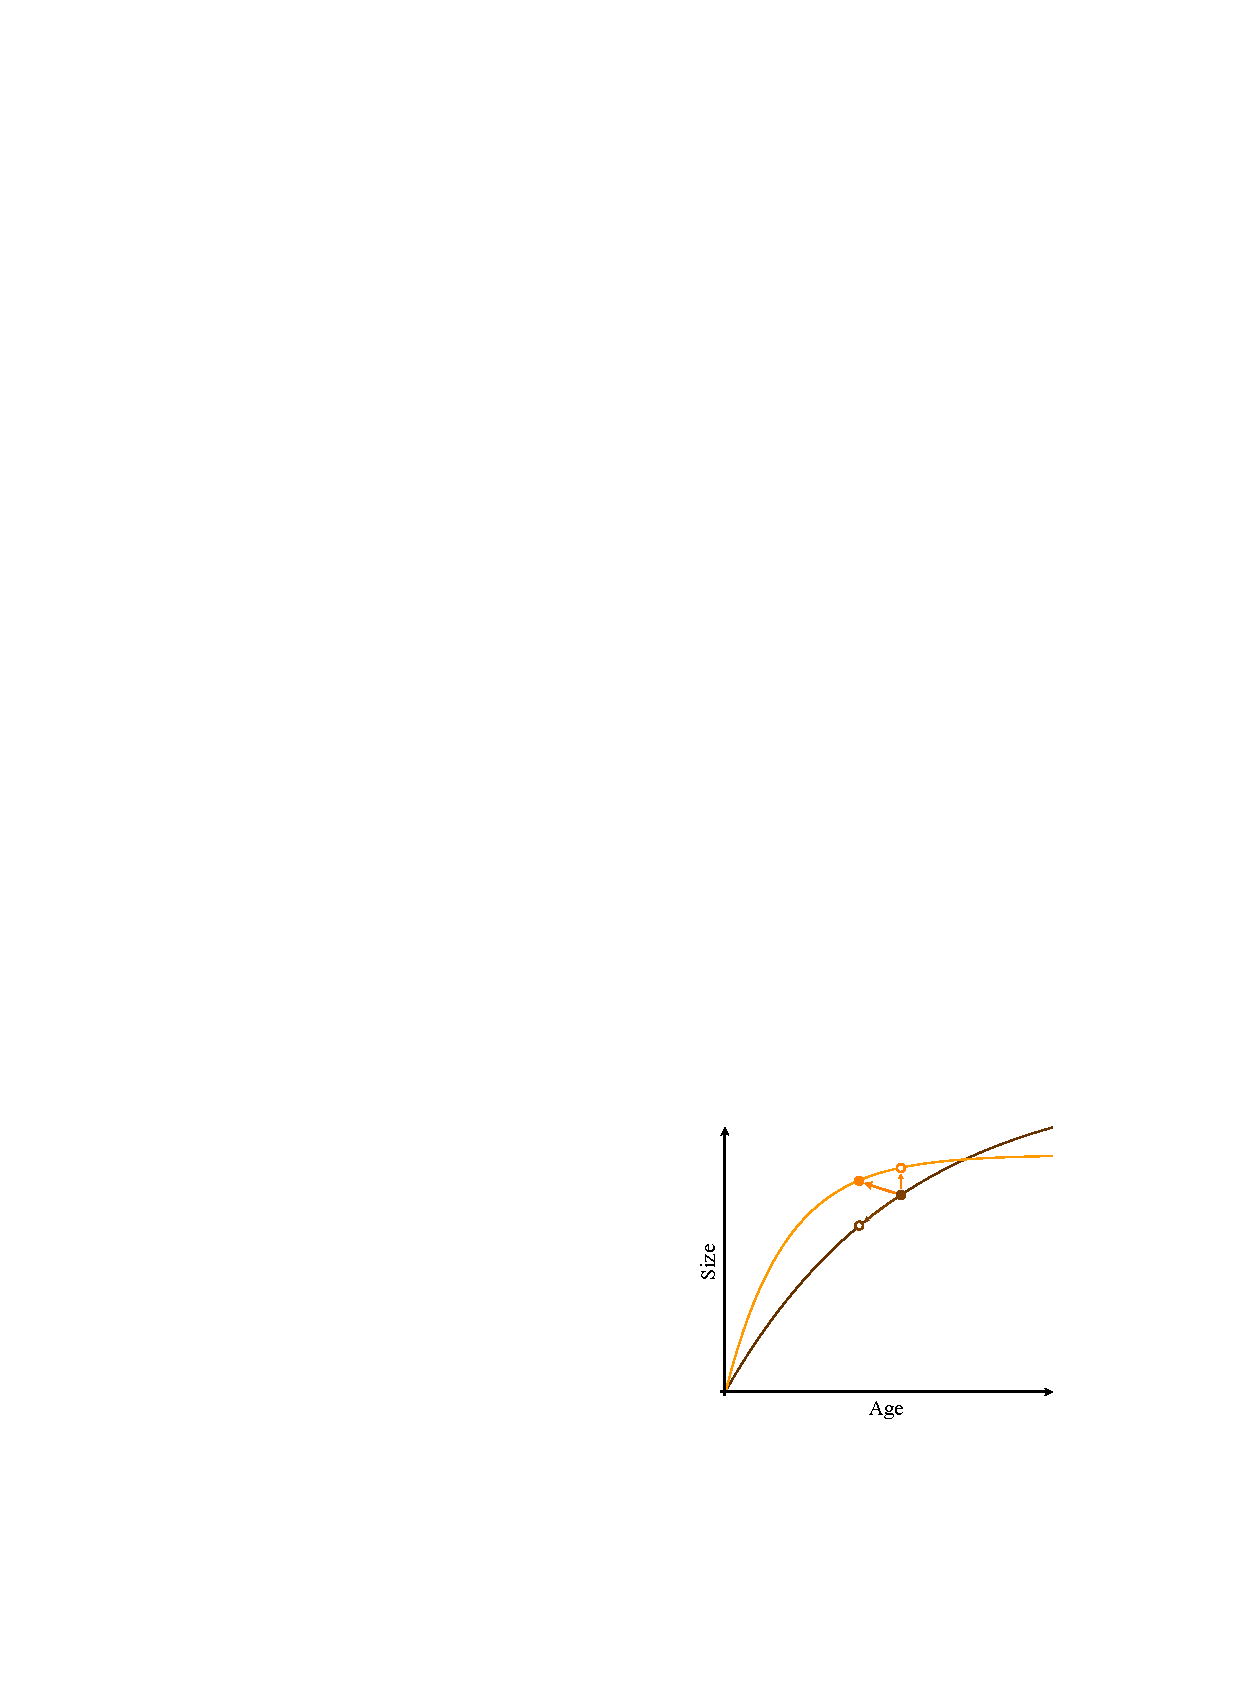
\includegraphics[width=0.5\textwidth]{1_CorpsDeThese/EA/Fig/ThermalNorm}
\caption[\lofimage{1_CorpsDeThese/EA/Fig/ThermalNorm}
Norme de réaction à la température]{Norme de réaction théorique à la
température \autocites[Figure 2]{ohlberger2013a}. Lors d'un changement de
température, le changement de taille à un âge donné (point orange plein) dépend
de l'importance relative de l'accélération de la croissance corporelle (point
orange vide), et de l'accélération du développement (point marron vide).}
\label{Fig:EA2}
\end{figure}

\subsection{Température et dynamique des populations}

La taille corporelle des individus et sa distribution étant un élément essentiel
dans la dynamique des populations, les variations de taille corporelle avec la
température ont des conséquences sur les dynamiques des populations et des
communautés. 

En effet, la température de l'environnement peut provoquer un changement de la
taille moyenne et de la structure d'une population. On retient en particulier
deux changements possibles : (i) la diminution de la taille à un âge donné avec
l'augmentation de la température (``size-at-age shift'') ; et (ii) le
changement de l'abondance relative des différents stades ou âges présents dans
la population (``structure shift''). Ces changements de structures sont causés
par l'intermédiaire de la croissance densité-dépendante, de la survie
taille-dépendante, de la compétition asymétrique entre les différentes
classes de taille et de la prédation taille-spécifique. Ces changements de
structures au niveau population peuvent ensuite se répercuter au niveau de la
communauté en affectant l'abondance relative de ses différentes espèces et son
organisation trophique. 

De plus, la température interagit fortement avec les mécanismes de densité
dépendance. Ainsi, il a par exemple été montré que le taux de croissance d'une
population peut augmenter avec la température si la population est présente en
faible densité, et à l'inverse diminuer avec la température si la population est
trop dense \autocites[chez le saumon royal][]{crozier2010a}. Dans le même
ordre d'idées, l'étude des registres de pêche du saumon d'atlantique a montré
qu'une température plus chaude était associée à des individus de grande taille si la
densité de la population était faible et l'inverse en climat froid
\autocites{huusko2012a}. 

La densité dépendance étant notamment liée à la compétition pour l'accès aux
ressources, qui elle-même dépend de la taille corporelle, l'augmentation de la
température peut provoquer une diminution de la taille moyenne dans une
population en favorisant des individus plus petits, plus compétitifs dans la
gestion de l'énergie s'il y a peu d'interférence
\autocites{persson1998a,ohlberger2012a}. Si la compétition par interférence est
forte, et si une grande taille corporelle fourni un avantage compétitif
conséquent, l'effet de la température sur la compétition devient alors plus difficile à
prédire.

Enfin, la température peut avoir des effets différentiels suivant le stade ou
l'âge des individus. En effet, il a été suggéré que des individus juvéniles
survivent plus facilement à un réchauffement que des individus plus grands ou
plus vieux \autocites{peck2009a}. Une augmentation de la température peut donc
avoir des effets différents suivant l'âge, le stade et la taille des individus,
ce qui se répercute sur la distribution de la taille dans la population, impactant
fortement sa dynamique. Ces changements de dynamique d'une population se
répercutent alors en cascade sur les communautés dont elles font partie, avec
des conséquences encore difficile à prévoir. 
